\section{Viewing}
Figure \ref{fig:detail_page} shows the detail page for DSPLearn. The detail page features a PDF viewer that supports an extensive range of PDF operations including print, download, zoom, rotate, search, and navigate. As seen, similar to the result page, the left sidebar also contains a hierarchical concept tree. The tree consists of concepts that are related to the section. There is also a search bar on top of the page.

\begin{figure}[!htbp]
  \centering
  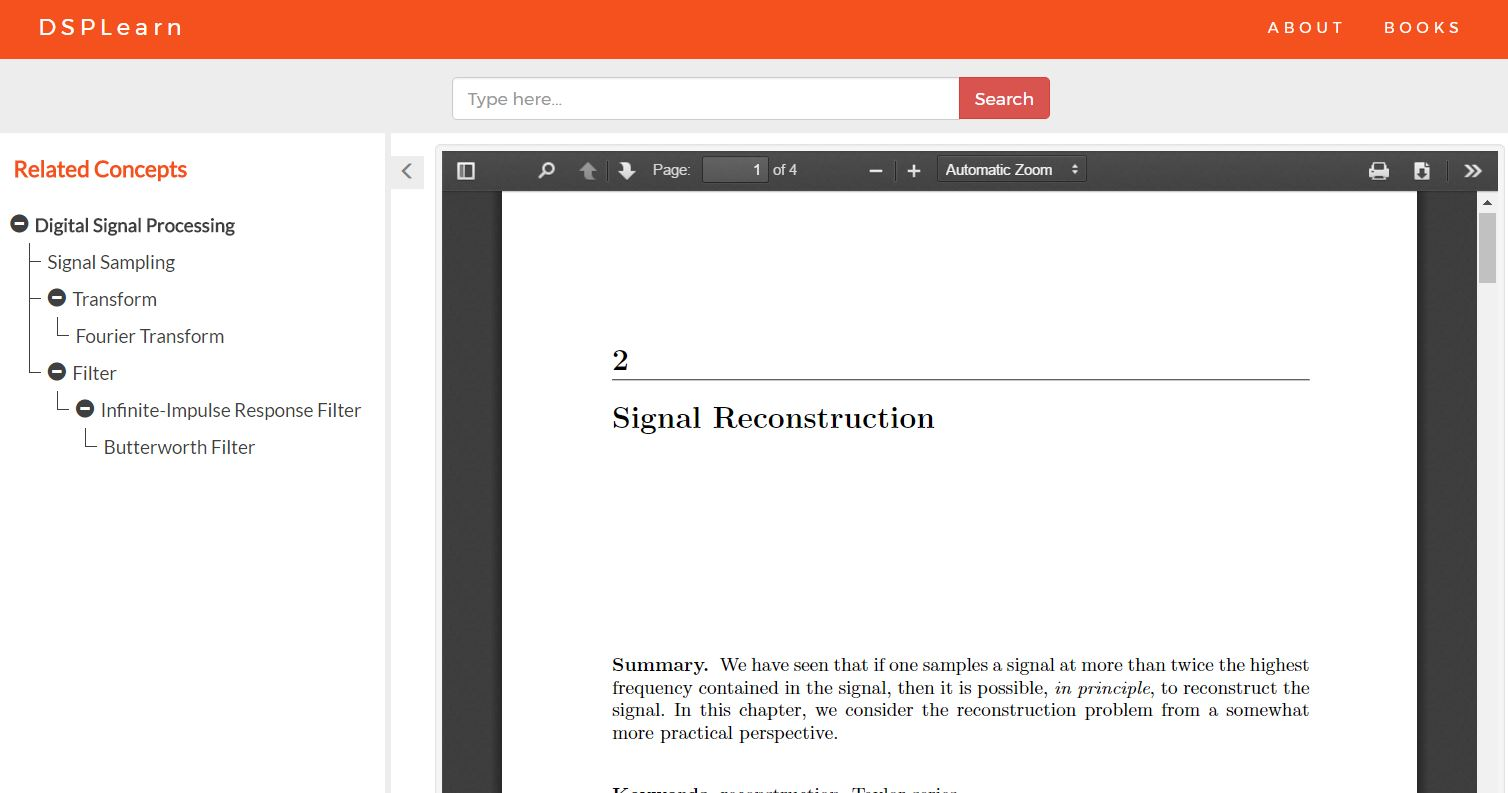
\includegraphics[width=\textwidth]{system_demonstration/demo_detail_page.jpg}
  \caption{DSPLearn Page for Viewing a Section}
  \label{fig:detail_page}
\end{figure}

The concept tree on the sidebar is also interactive. A dialog would pop up when users select a concept (\ref{fig:detail_popover}). Users may choose to highlight terms in the PDF document that are mapped to the selected concepts in the tree.

\begin{figure}[!htbp]
  \centering
  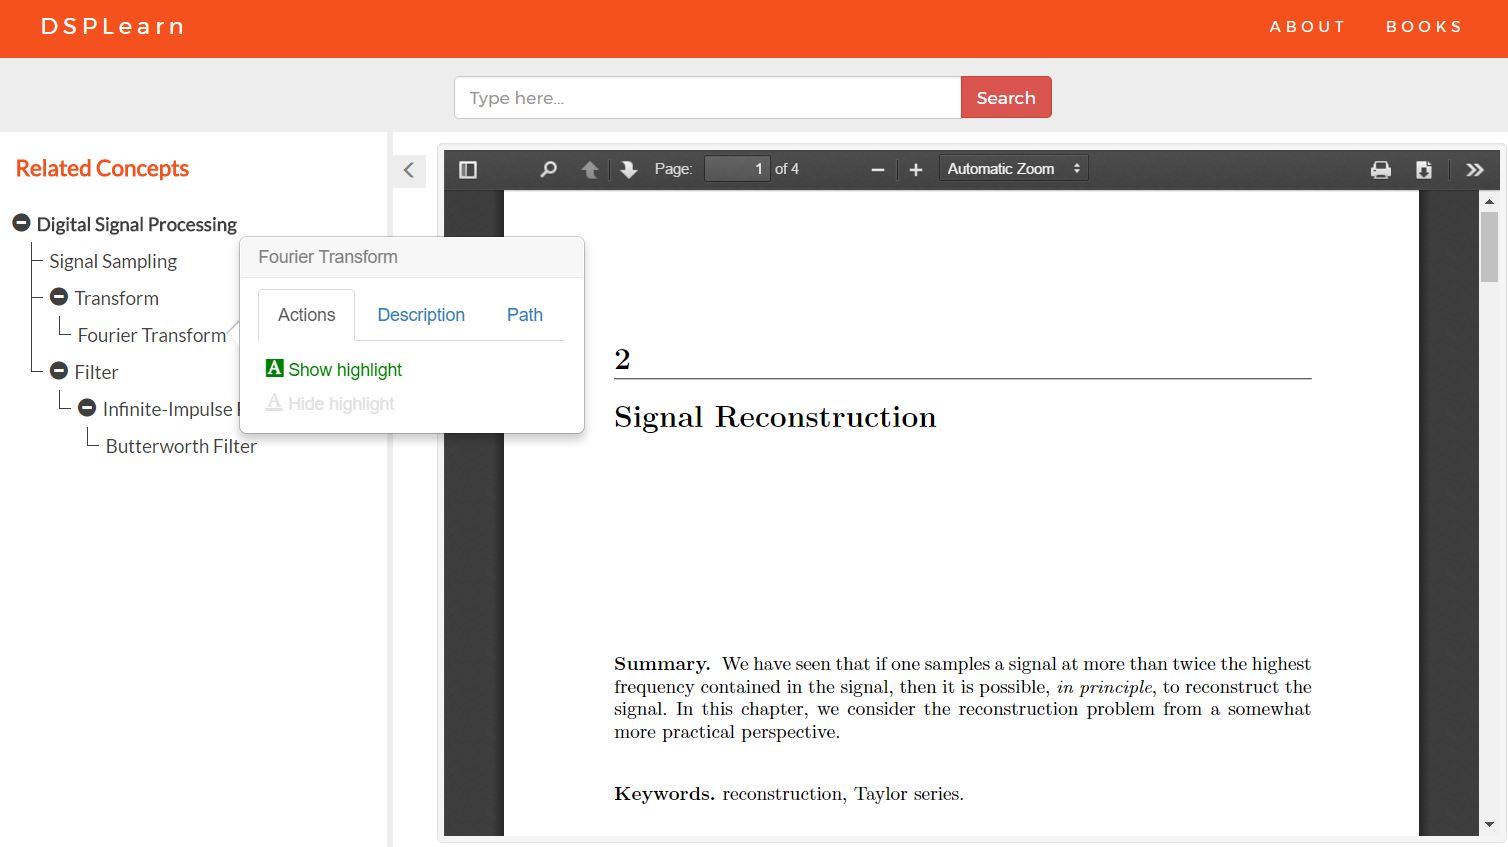
\includegraphics[width=\textwidth]{system_demonstration/demo_detail_popover.jpg}
  \caption{Concept Popover in Detail Page}
  \label{fig:detail_popover}
\end{figure}

The dialog also has 3 tabs - \enquote{Actions}, \enquote{Description}, and \enquote{Path}. There are 2 actions to choose from - \enquote{Show highlight} and \enquote{Hide highlight}. 
All terms are not highlighted by default. When \enquote{Show highlight} is chosen, the concept would be in green, as shown in Figure \ref{fig:detail_highlight}. When \enquote{Hide highlight} is chosen, the concept would revert back to normal.

\begin{figure}[!htbp]
  \centering
  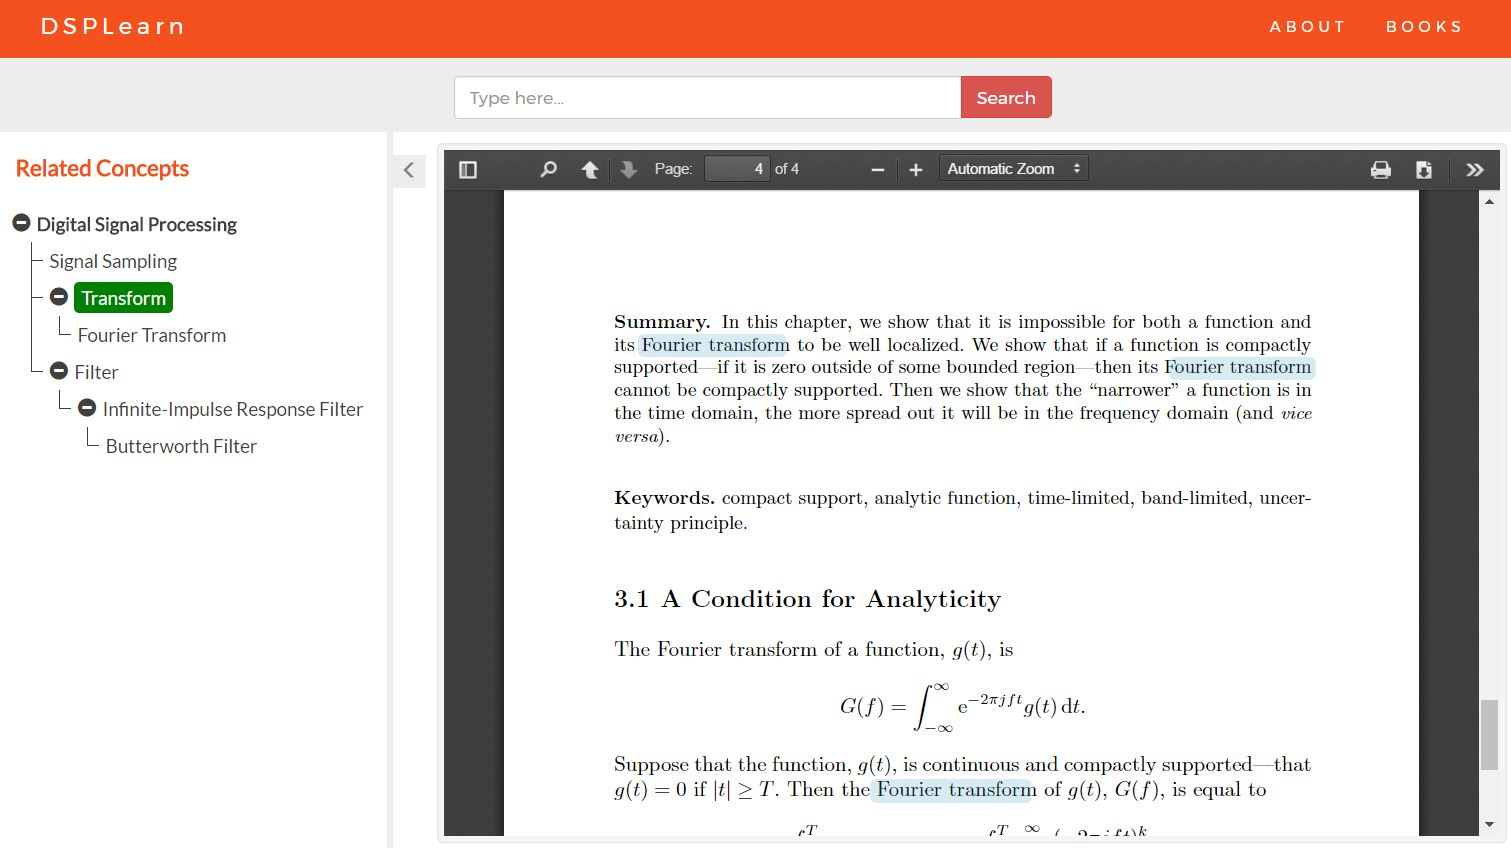
\includegraphics[width=\textwidth]{system_demonstration/demo_detail_highlight.jpg}
  \caption{Term Highlighting in PDF}
  \label{fig:detail_highlight}
\end{figure}

In Figure \ref{fig:detail_highlight}, all terms mapped to the concept \enquote{Transform} are highlighted in the PDF document. The section ID for this document is 2192. Based on the ontology and term-to-concept mappings in Figure \ref{fig:django_admin_concept_mapping}, only the second entry in the \texttt{Concept mappings} table is applicable. In the second entry, it says that the first, second, third, and fifth occurrences of the case-insensitive term \enquote{fourier transform} are mapped to the concept \enquote{Fourier Transform}. Since \enquote{Fourier Transform} is a child concept of \enquote{Transform}, as defined in the ontology (Figure \ref{fig:sfig:admin_concepts}), these 4 occurrences of terms are also mapped to the concept \enquote{Transform}.

The PDF snippet in Figure \ref{fig:detail_highlight} shows the highlights of the second, third, and fifth occurrences of the term \enquote{fourier transform}. As noted, the fourth occurrence of the term is not highlighted as expected.